%%%%%%%%%%%%%%%%%%%%%%%%%%%%%%%%%%%%%%%%%%%%%%%%%%%%%%%%%%%%%%%%
%%                          CHAPTER 2                         %%
%%%%%%%%%%%%%%%%%%%%%%%%%%%%%%%%%%%%%%%%%%%%%%%%%%%%%%%%%%%%%%%%
\chapter{\ak\ Synchroniser}
A synchroniser is a vertex that produces output messages based on a potentially unlimited history of input messages read from its input channels. In order to do this, a synchroniser maintains an internal state and makes state transitions. The states and transitions between them define which channels are read and in what order depending on the channel status (available, not available) and optionally the content of the messages. Messages received in various states can be stored in the synchronisation storage with the single purpose to retrieve them in another state and to use them in output messages.

    \section{Mathematical Model}
From the mathematical point of view a synchroniser is a pair $(\Phi, \; \Pi)$, where
  \begin{itemize}
  \item[] $\Phi = (A, \; S, \; T)$ -- nondeterministic state machine:
    \begin{itemize}
    \item[] $A \subseteq C \times P$ -- the alphabet of events, $C$ -- set of synchroniser input channels, $P$ -- set of predicates on channel messages. An event $(c, \; p) \in A$ represents the reception of a message on channel $c$ that satisfies predicate $p$,
    \item[] $S \supseteq \{s_{0}\}$ -- set of abstract states, $s_{0}$ -- start state,
    \item[] $T \: : \: A \times S \to S$ -- transition matrix.
    \end{itemize}
  \item[] $\Pi \: : \: S \times \Omega \to V$ -- path functional that defines the synchroniser output:
    \begin{itemize}
    \item[] $\Omega$ -- the set of output channels,
    \item[] $V$ -- the set of message values \cite{astrakahn}.
    \end{itemize}
  \end{itemize}

In a state $s_{k}$ the functional is based on the retrospective sequence of transitions from the most recent visit to the start state $s_{0}$ to $s_{k}$:
  \begin{itemize}
  \item[] $(s_{0}, c_{0}), \: (s_{1}, c_{1}),... \: (s_{k}, c_{k})$, where
    \begin{itemize}
      \item[] $s_{0}$ -- start state,
      \item[] $c_{i} \in C$, $0 \le i \le k$ -- the channel that caused the transition from the state $s_{i}$.
    \end{itemize}
  \end{itemize}

Let $\mu_{i}$ be the message received in the transition from the state $s_{i}$. Then
  \begin{itemize}
  \item[] $\Pi \; (s_{k}, \omega_{m}) = \psi_{\sqcap} \; \{\mu_{i} \: | \: \rho_{ki}^{m} \; (s_{i}), \: 0 \le i \le k\}$, where
    \begin{itemize}
      \item[] $\rho_{ki}^{m}$ -- selection predicate that defines $\Pi$,
      \item[] $\psi_{\sqcap}$ -- the operator that coerces the messages in the operand set to their joint greatest subtype.
    \end{itemize}
  \end{itemize}

From the above, the synchroniser is fully defined by two functions:
  \begin{enumerate}
  \item The transition matrix $T$

The state machine can have a regular structure whereby many transitions can be defined at once by a formula with some limited range integer variables. For example, a machine with 8 states could have a transition matrix defined thus: $S_{k \; mod \; 8} \to S_{k+1 \; mod \; 8}$.

In order to be able to use regular structures, \ak\ allows synchronisers to declare \emph{state} variables.

\textbf{Example: the counter synchroniser}  Counter emits every $n$-th message received in its input channel to the output channel. The transition diagram for the counter synchroniser for $n = 3$ is given in Figure \ref{fig:counter}.a.

Mathematical model $S_{counter_{3}} = (\Phi, \; \Pi)$, where
  \begin{itemize}
  \item[] $\Phi = (A, \; S, \; T)$,
    \begin{itemize}
    \item[] $C = (a)$, $P = (true)$, $A = C \times P = ((a, \; true))$,
    \item[] $S = (s_{0}, \; s_{1}, \; s_{2})$, $s_{0}$ -- start state,
    \item[] $T$:
      \begin{tabular}{c|c|c|c}
      $A$ \textbackslash $S$ & $s_{0}$ & $s_{1}$ & $s_{2}$\\
      \hline
      $(a, \; true)$ & $s_{1}$ & $s_{2}$ & $s_{0}$\\
      \end{tabular}
    \end{itemize}
  \item[] $\Pi \: : \: S \times \Omega \to V$,
    \begin{itemize}
    \item[] $\Omega = (c)$,
    \item[] $V = (a)$
    \end{itemize}
  \end{itemize}

An output message is emitted when a transition happens from the state $s_{2}$. This state is reached in a single path:
  \begin{itemize}
  \item[]
$W_{0} = ((s_{0}, \; a), \: (s_{1}, \; a), \: (s_{2}, \; a))$
% fixed rho{1i}^{c} to rho{2i}^{c}
$\Pi \; (s_{2}, c) = \psi_{\sqcap} \; \{\mu_{0} = a \: | \: \rho_{20}^{c} \; (s_{0}) = 0, \mu_{1} = a \: | \: \rho_{21}^{c} \; (s_{1}) = 0, \mu_{2} = a \: | \: \rho_{22}^{c} \; (s_{2}) = 1\}$, $k = 1$, $i = 0,1,2$ 
  \end{itemize}

The state machine behind the counter has a regular structure, and for this synchroniser all its transitions may be defined with a single formula: $S_{k \; mod \; 3} \to S_{k+1 \; mod \; 3}$. Considering this, the transition matrix $T$ would be:
  \begin{tabular}{c|c}
  $A$ \textbackslash $S$ & $S_{k \; mod \; 3}$\\
  \hline
  $(a, \; true)$ & $S_{k+1 \; mod \; 3}$
  \end{tabular}

Some possible transition diagrams of the counter synchroniser are given in Figure \ref{fig:counter}. The diagram \ref{fig:counter}.a represents the unrolled regular structure of the synchroniser. However, this representation is inconvenient when $n \gg 1$. The transition diagram \ref{fig:counter}.a can be folded using state variables. Two possible variants are shown in figures \ref{fig:counter}.b and \ref{fig:counter}.c. The state variable $c$ acts as an induction variable in a while loop with the exit condition $c \ge 3$.

  \begin{figure}[here]
  \centering
  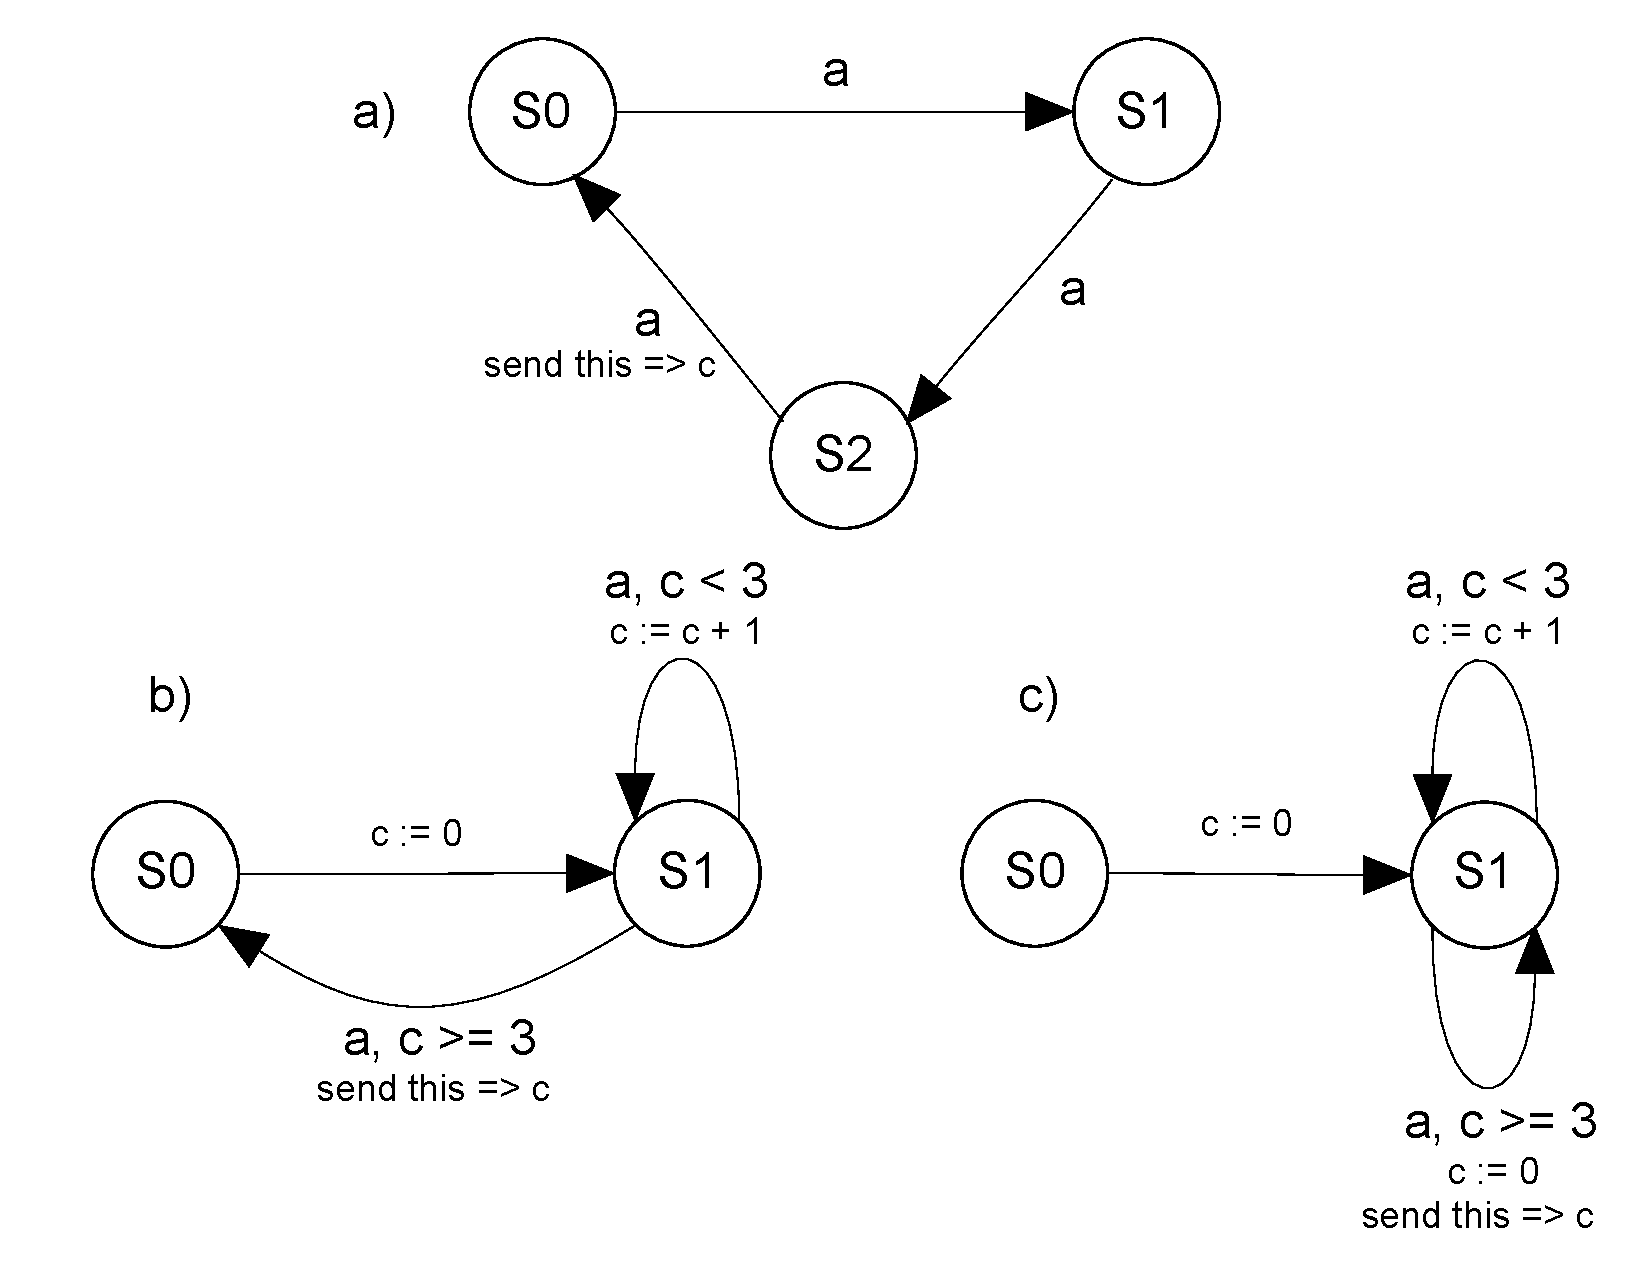
\includegraphics[scale=0.4]{figs/counter.pdf}
  \caption{The transition diagrams of the counter synchroniser.}
  \label{fig:counter}
  \end{figure}


  \item The selection predicate $\rho$

In a given state $k$ for each output channel $\omega_{m}$ we note all $i$ on which $\rho_{ki}^{m}$ is true. Those message values must be stored in a previous state and recalled in state $k$. It is expected that the boolean vector $\omega_{i} = \rho_{ki}^{m}$ has only very few true elements.

Consequently the storage mechanism that \ak\ provides for synchronisers is in the form of individual \emph{store} variables. The type of a store variable is determined when a variable is assigned.

\textbf{Example: the binary zip synchroniser}  Zip2 receives messages on its input channels and sends their concatenation to the output channel. In the resulting concatenation there's exactly one message from each input channel and those messages are ordered as they received.

The zip2 transition diagram is given in Figure \ref{fig:zip2}. The message received in the current transition is referred by a keyword \emph{this}. $ma$ and $mb$ are the store variables associated with the input channels $a$ and $b$ respectively. The statement \emph{send} indicates a sending of a message to an output channel.

  \begin{figure}[here]
  \centering
  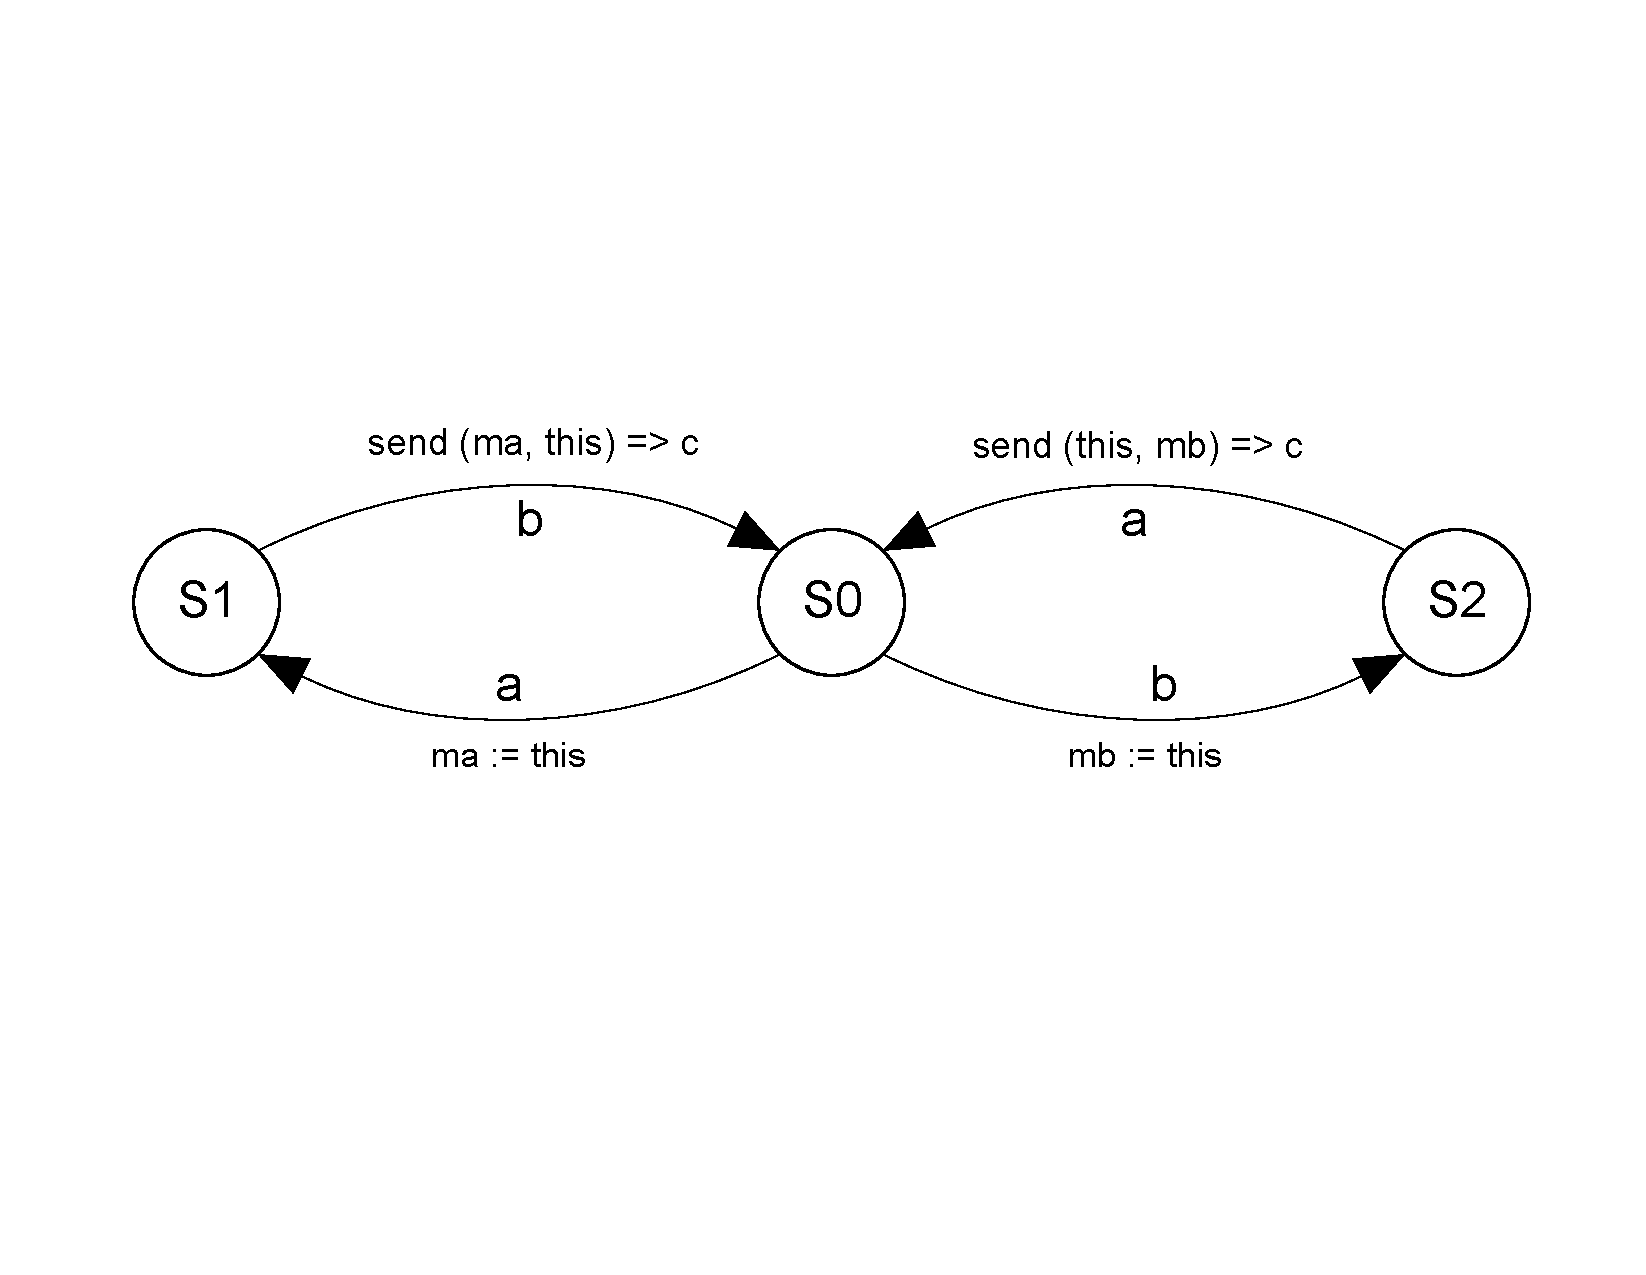
\includegraphics[scale=0.4]{figs/zip2.pdf}
  \caption{The transition diagram of the zip2 synchroniser.}
  \label{fig:zip2}
  \end{figure}

Mathematical model $S_{zip2} = (\Phi, \; \Pi)$, where
  \begin{itemize}
  \item[] $\Phi = (A, \; S, \; T)$,
    \begin{itemize}
    \item[] $C = (a, \; b)$, $P = (true)$, $A = C \times P = ((a, \; true), \: (b, \; true))$,
    \item[] $S = (s_{0}, s_{1}, s_{2})$, $s_{0}$ -- start state,
    \item[] $T$:
      \begin{tabular}{c|c|c|c}
      $A$ \textbackslash $S$ & $s_{0}$ & $s_{1}$ & $s_{2}$\\
      \hline
      $(a, \; true)$ & $s_{1}$ & $s_{1}$ & $s_{0}$\\
      \hline
      $(b, \; true)$ & $s_{2}$ & $s_{0}$ & $s_{2}$\\
      \end{tabular}
    \end{itemize}
  \item[] $\Pi \: : \: S \times \Omega \to V$,
    \begin{itemize}
    \item[] $\Omega = (c)$,
    \item[] $V = ((a, \; b), \: (b, \; a))$
    \end{itemize}
  \end{itemize}

An output message is emitted when a transition happens either from the state $s_{1}$ or the state $s_{2}$. These states are reached in two paths:
  \begin{itemize}
  \item[]
$W_{0} = ((s_{0}, \; a), \: (s_{1}, \; b))$

$\Pi \; (s_{1}, c) = \psi_{\sqcap} \; \{\mu_{0} = a \: | \: \rho_{10}^{c} \; (s_{0}) = 1, \mu_{1} = b \: | \: \rho_{11}^{c} \; (s_{1}) = 1\}$, $k = 1$, $i = 0,1$
  \item[]
$W_{1} = ((s_{0}, \; b), \: (s_{2}, \; a))$

$\Pi \; (s_{2}, c) = \psi_{\sqcap} \; \{\mu_{0} = b \: | \: \rho_{20}^{c} \; (s_{0}) = 1, \mu_{2} = a \: | \: \rho_{22}^{c} \; (s_{2}) = 1\}$, $k = 2$, $i = 0,2$ 
  \end{itemize}
  \end{enumerate}


\section{The language for \ak\ synchroniser}
We develop the language according to chosen message protocol. The protocol restricts anything but a $choice$ termed message trevelling in channels. This the syntax $on a.(x,y, ...)$ is not needed with this protocol. We may include this syntax as a syntax sugar for $uniq$ when choice has just one alternative. Originally this syntax was intended for records in channels. However, the chosen protocal doesn't allow it. For example if we want to extend the protocol for lists to travel in channels, we need to define the union of lists, possibly as a construct with 2 nested lists $(union l_1 l_2)$ and we need to extend the protocol to encode this construct. For record and choice union is easy to define. If no labels in $t_1$ and $t_2$ intersect then the resulting record of choice has all the labels from $t_1$ and $t_2$ with their values: $t = union \; t_1 \: t_2 = union \; \{a:t_a\} \: \{b:t_b\} = \{a:t_a, \: b:t_b\}$. When labels intersect, it is the deal for CAL solver to resolve with option to take (it should consider flow inheritance). The synchroniser just leaves it to be a union of terms:

For example for Choice: $union \; (: \: a:t_a \: :) \: (: \: a:t_b \: :) = (: \: a:union \: t_a, \: t_b \: :)$.
Same for record.


\subsection{Synchroniser code}
%% TODO fix 'channel connected to the port x' to channel x
%% Insert a footer that explains that 'channel x' is short for 'channel connected to the port x'
An \ak\ synchroniser is a finite state machine, therefore the basic building blocks of a synchroniser program are states and transitions. A state of a synchroniser is fully defined by the corresponding state of the finite state machine and the values of the state variables. A transition is the act of moving to another state which is initiated by a triggering event. A triggering event for the synchroniser transition is an arrival of a message to the associated channel. The message may be required to have a specific structure. In addition, a transition may be guarded by special conditions on the values of the state variables. If the conditions are satisfied the transition fires, otherwise it is cancelled.

Once a transition is known to fire, optional actions may be performed before the underlying state machine makes the move. These actions include changing the state and store variable values and sending messages to the output channels. In order to change the state and store variables, the synchroniser language provides state and store expressions over them.

This section gives an overview of the \ak\ synchroniser programming language. The formal grammar of the \ak\ synchroniser is provided in Appendix \ref{sync_syntax}.

  \subsubsection{Program structure}
A synchroniser program consists of a header followed by the synchroniser's body wrapped in braces. The begining of a synchroniser program is indicated by the keyword $synch$.

The header of a synchroniser program contains the synchroniser's name and the channel signature. The name is an ASCII string that follows the C convention.

The body of the synchroniser lists the state and store variables declarations and the states of the underlying finite state machine. Each state is defined by a list of transitions. Each transition lists its triggering condition which includes an optional guarding state expression, an optional list of actions, and, finally, the destination state.

%  \subsection{Macros}
%%%
%%% We removed macros from the language. The compiler must invoke a preprocessor to expand them.
%%%
%The synchroniser language provides macros to avoid having to trivially alter synchroniser programs. Macros are specified in brackets between the synchroniser's name and its channel signature. An example of a configurable synchroniser can be found in \cite{astrakahn}.

  \subsubsection{Channel signature}
The channel signature defines the input channels and the output channels of the synchroniser and their bracketing depths. The synchroniser header (Fig. \ref{min_sync_head}) declares the synchroniser $min$ with two input channels that are connected to the ports $a$, $b$ and two output channels that are connected to the ports $c$, $d$. If the bracketing depths of the channels are not specified, they are assumed to be 0. Thus, the bracketing depth of the channel $a$ is 0.

The input channel depth $-1$ indicates that the input channel is ignored in the synchroniser program. The output channel with the depth $-1$ must not have data sent to them.

\begin{figure}[h!]
\begin{lstlisting}[frame=single]
synch min (a, b:p | c:2, d:p+1)
\end{lstlisting}
\caption{The synchroniser header}
\label{min_sync_head}
\end{figure}

%% TODO remove read-only state variables

The \ak\ synchroniser allows to declare constant and configurable integer depths for the input and output channels. In addition, the depth of the output channel can be specified with an integer shift to the configurable input channel depth.

The input channels are required to have the bracketing depths specified in the signature. Thus, the channel $a$\footnote{channel connected to the port $a$ is meant. Later on we will call a channel connected to the port $x$ channel $x$ for short} of the $min$ synchroniser must have zero bracketing depth. The channel $b$ has a configurable bracketing depth $p$. Actual values of configurable bracketing depths of input channels are determined by the \ak\ compiler. %Once defined in the signature, configurable bracketing depths may be used in state expressions. They are interpreted as read-only state variables.

The output channels of a synchroniser are guaranteed to have the bracketing depths specified in the channel signature. Thus, the synchroniser $min$ must send messages to the output channel $c$ at the depth 2 and optionally at the depths $0$, $1$. The output channel $d$ must have the bracketing depth $p+1$ that is the depth of the input channel $b$ increased by $1$.


%% TODO Move all the type details to the implementation details
%% TODO The width of int type is declared explicitly to reduce the number of potential states of automata.
  \subsubsection{Variable declaration}
%% Add about state and store variables initialisation.
%% state int(8) a, b=1, c=8; // assignes a=0 b=1 c=9
%% enum (a,b,c) foo, bar=a;  // assignes foo=0 bar=a
The beginning of state variables declaration is indicated by the keyword $state$. A state variable may be either a unsigned integer of the constant width or a C-style enumeration. State and store variables names are user-defined indentifiers. A user-defined identifier is an ASCII string that follows the C convention.

%% TODO Should move width determining to the implementation detail
Line 1 in Fig. \ref{sync_statevar} declares state variables $a$, $b$, $c$ of width 4. Thus, all three variables are declared to have integer values in the range $[0; 15]$. Generally, a state variable of width $n$ has integer values in the range $[0; 2^{n}-1]$.

The state variable $foo$ that is declared in the line 2 in Fig. \ref{sync_statevar} can only be assigned the values $d$, $e$ and $f$ specified in the enumeration. The enumeration values are integer constants. If the values are not specified explicitly, they are assigned consequtive positive integers starting with 0.
%The width of the $int$ type is $\lceil \log_{2}{n} \rceil + 1$, where $n$ is the number of values in the enumeration.
Thus, the variable $foo$ has integer values $d=0$, $e=1$ and $f=2$. % of the width $\lceil \log_{2}{3} \rceil + 1 = 3$. If the values are specified explicitly, the width is determined as $\lceil \log_{2}{(m+1)} \rceil + 1$, where $m$ is the biggest value in the enumeration. For the variable $bar$ declared in line 3 of Fig. \ref{sync_statevar} $m=4$ and the width is $\lceil \log_{2}{(5)} \rceil + 1 = 4$.


The values can be specifed explicity (see line 3 in Fig. \ref{sync_statevar})

Integer state variables and enum values can be mixed freely in state expressions. Enum values are interpreted as integer constants.%read-only integer state variables. % constant integers!

\begin{figure}[h!]
\lstset{numbers=left, numberstyle=\small, stepnumber=1, numbersep=8pt}
\begin{lstlisting}[frame=single]
state int(4) a, b, c;
state enum(d, e, f) foo;
state enum(x = 1, y = 2, z = 4) bar;
store msg_a, msg_b;
\end{lstlisting}
\caption{State and store variables declaration}
\label{sync_statevar}
\end{figure}

Store variables declaration begins with a keyword $store$. Line 4 in Fig. \ref{sync_statevar} declares state variables $msg\_a$ and $msg\_b$. Store variables do not need explicit type specification; their types are determined on the first assignment to the variable.

All the state and store variables are global to all the synchroniser states.


  \subsubsection{States and transitions}
States and transitions of the synchroniser define which channels are read and in what order. Fig. \ref{zip_struc} presents the code of the binary zip synchroniser's state machine. Line 1 declares the start state of the synchroniser. The $on$ clause indicates the beginning of the transitions list. In the start state the zip2 synchroniser acceptes messages from both input channels $a$ and $b$. State and store expressions associated with the transition and the destination state are specified in the braces.

\begin{figure}[h!]
\lstset{numbers=left, numberstyle=\small, stepnumber=1, numbersep=8pt}
\begin{lstlisting}[frame=single]
start {
  on:
    a { goto s1;    }
    b { goto s2;    }
}
s1 {
  on:
    b { goto start; }
}
s2 {
  on:
    a { goto start; }
}
\end{lstlisting}
\caption{State machine of the zip2 synchroniser}
\label{zip_struc}
\end{figure}

When the zip2 synchroniser is in the start state and it receives a message from the channels connected to the port $a$, the underlying state machine makes a transition to the state $s1$. In this state the synchroniser can only receive messages from channel $b$ since there's no transition triggered by channel $a$ and defined in this state. When the message on channel $b$ is received, the state machine makes a transition to the start state. Lines 10-13 define similar behaviour in state $s2$.

%% Change 'scopes'. 'Blocks' probably
The synchroniser language supports top-down prioritised transition scopes. They are indicated with the $elseon$ keyword. A synchroniser in state $foo$ in Fig. \ref{sync_scope} acceptes messages from channels connected to the ports $a$, $b$, $c$ and $d$. When no destination state is specified for a transition, a synchroniser makes the transition to the current state. If all channels are ready at the same time in state $foo$, the synchroniser processes messages from either channel $a$ or $b$ first. When all messages from channels connected to the ports $a$ and $b$ are processed the synchroniser receives messages from channels connected to the port $c$. If there're no messages in channels $a$, $b$ and $c$ the synchroniser receives messages from the channel $d$.

\begin{figure}[h!]
\lstset{numbers=left, numberstyle=\small, stepnumber=1, numbersep=8pt}
\begin{lstlisting}[frame=single]
foo {
  on:
    a { }
    b { }
  elseon:
    c { }
  elseon:
    d { }
}
\end{lstlisting}
\caption{Prioritised transition scopes}
\label{sync_scope}
\end{figure}


  \subsubsection{State expressions}
State expression is a combination of integer constants, state variables and operators, which computes and produces an integer value. The interpretation of a state expression follows C rules of precedence and association. State expressions can be assigned to state variables. In assumption that the output channel is infinite a synthetic example in Fig. \ref{sync_state_exp} counts the number of messages received from channel $a$ between the arrivals of messages in channel $b$. Line 1 declares the 8-bit integer $count$ and initialises it with 0. When a message from $a$ is received the value of $count$ increases by 1 (see line 5).

\begin{figure}[h!]
\lstset{numbers=left, numberstyle=\small, stepnumber=1, numbersep=8pt}
\begin{lstlisting}[frame=single]
state int(8) count = 0;
foo {
  on:
    a {
      set count = [count + 1];
    }
  elseon:
    b {
      set n = [count], count = [0];
      send count:[n] => c;
    }
}
\end{lstlisting}
\caption{Use of state variables and expressions}
\label{sync_state_exp}
\end{figure}

When a message from channel $b$ is received the value of $count$ is stored in the temporary variable $n$, set to 0 and then $n$ is sent to the output channel.

The variable $n$ does not have to be declared and is considered alias for the integer expression. Temporary variables are available until the state machine of a synchroniser makes the next move.


  \subsubsection{Triggering of a transition}
The channel name on its own stands for the availability predicate for the corresponding channel, i.e. the condition that a message of any kind is available. Whether a transition takes place depends on the channel status and optionally the content of the messages.

When a message is received on a channel, it can be matched with a pattern in order to extract parameters needed to select a specific transition. In line 3 of Fig. \ref{sync_trans} it is checked whether a message received from the input channel $a$ is a unique choice. Then the unique record is checked whether it contains a label $x$. If it does, the contents of $x$ are stored in a temporary variable $x$. The tail of the message, i.e. all label-term pairs except for the term labeled $x$, is stored in a temporary variable $t$. Both $x$ and $t$ are available until the state machine makes the next move. %read-only?

%TODO: Fix; everything in $.?v(.... || tail)$ before $||$ are integers.
\begin{figure}[h!]
\lstset{numbers=left, numberstyle=\small, stepnumber=1, numbersep=8pt}
\begin{lstlisting}[frame=single]
foo {
  on:
    a.(x || t)  { }
    a.?v        { }
    a.?v(x, y)  { }
    a.@[k]      { }
}
\end{lstlisting}
\caption{Message content extraction}
\label{sync_trans}
\end{figure}

To support message formats where several variants of a message are possible, a qualifier \begin{bf}?\end{bf}$\alpha$ is available as an input condition. It qualifies input messages as belonging to $\alpha$ variant. In line 4 of Fig. \ref{sync_trans} it is checked whether a message received from channel $a$ belongs to the variant $v$. In line 5 it is checked whether a message that belongs to the variant $v$ contains only two records labeled $x$ and $y$. 

A channel carries a stream that consists of messages and possibly segmentation marks. In line 6 in Fig. \ref{sync_trans} a message is checked if it is a segmentation mark of the depth $k$. The depth of a segmentation mark can be a state expression.

Several different channels can be tested in any given state, however, once the readiness of a channel was established, the synchroniser is committed. Hence the set of conditions applied to the message on any input channel must be exhaustive. In Fig. \ref{sync_trans} it is not, because there no pattern for messages that do not contain label $x$, do not belong to variant $v$ and are not a segmentation mark of depth $k$ at the same time. In this case the final clause $a$\begin{bf}.else;\end{bf} is assumed. This clause discards the input message and transitions the synchroniser back to its current state.

A transition can be guarded by a state expression. In this case the transition fires only if the guarding expression evaluates to true. The synchroniser in Fig. \ref{sync_g_state_exp} sends every 256-th message to the output channel. In line 1 the 8-bit state variable $i$ is declared and initialised with 0. The variable is incremented every time a message from channel $a$ is received, except for when it reaches 255, in which case it is reset to 0 and the received message is sent down the channel $c$. 

Values that are matched from the message can be used in guarding state expressions.
\begin{figure}[h!]
\lstset{numbers=left, numberstyle=\small, stepnumber=1, numbersep=8pt}
\begin{lstlisting}[frame=single]
state int(8) i;
start {
  on:
    a & [i < 255] {
      set i = [i + 1];
    }
    a & [i = 255] {
      set i = [0];
      send this => c;
    }
}
\end{lstlisting}
\caption{Use of guarding state expressions}
\label{sync_g_state_exp}
\end{figure}


  \subsubsection{Store expressions and sending messages}
%% TODO Probably fix it after writing about CAL terms.
Store expression is a mechanism to combine data. Data are typed in \ak\. Types are CAL terms. Store expression concatenates data and therefore results in the data of a valid CAL type. The result of the store expression can be either stored in a store variable or sent down the output channel.

The example in Fig. \ref{sync_send} demonstrates the use of store expressions and the $send$ clause. In the start state the synchroniser receives messages from channel $a$ that has label $n$ in it. In line 5 the value under label $n$ is incremented and stored in the store variable $ma$ under label $n$ together with the tail $t$. The syntactic sugar for defining a record is supported. The operator $'$ applied to the variable $x$ creates the record $'x': value(x)$.

%% TODO Provide a more convincing example for 'id and this
\begin{figure}[h!]
\lstset{numbers=left, numberstyle=\small, stepnumber=1, numbersep=8pt}
\begin{lstlisting}[frame=single]
store ma;
start {
  on:
    a.(n || t) {
      set ma = (n:[n+1] || t);
      goto s1;
    }
}
s1 {
  on:
    b {
      send ma || this => c;
      goto start;
    }
}
\end{lstlisting}
\caption{Use of store expressions and the $send$ clause}
\label{sync_send}
\end{figure}

A message received on a channel is referred to by the keyword $this$ within the active transition. In state $s1$ the synchroniser receives messages from channel $b$. When a message is received, it is concatenated with the store variable $ma$ (see line 12) and sent to the output channel $c$.



\section{Execution order of synchroniser\label{execod}}
\begin{itemize}
\item Fairness policy
In a certain state both input channels may be ready, but a state machine receives input symbols one at a time. Which transition will be triggered under such circumstances is defined by the fairness policy: the coordinator will ensure that when more than one transition is possible in a given state, all choices will be made with the same frequency.

\item Non-deterministic $goto$

The purpose of non-deterministic gotos comes from the requirement that the synchroniser must not block the execution. If non-deterministic goto is the case then the synchroniser makes a fair transition to the state that sends messages to the channel that is not blocked.

In other words, the synchoniser avoids to make transitions to the states that send messages to blocked channels.


\item Algorithm of the execution of synchronisers
on-elseon execution order, dead $elseon$ code with $\langle chan \rangle .else$
\end{itemize}


\section{The implementation of the $aksync$ compiler}
In this section we describe the implementation of the \ak\ synchroniser compiler $aksync$. At the current stage of the \ak\ software stack development the $aksync$ compiler is highly integrated into the \ak\ runtime system prototype. Like the runtime system the $aksync$ compiler is implemented in Python. It generates an intermediate representation of the synchroniser program that is passed to the synchroniser runtime.

Lexical and syntax analysers are implemented using PLY \cite{ply} - an implementation of lex and yacc parsing tools for Python. Semantic analyser performs syntactic and type checking. Code generator emits synchroniser's runtime data structure and derives synchroniser's CAL passport.


\subsection{Lexical analysis}
  \subsubsection{Lexical analyser}
The lexical analyser reads the stream of characters making up the source program and groups the characters into lexemes. For each lexeme, the lexical analyser produces a token of the form $\langle name, \: value \rangle$ that it passes to the syntax analyser. For tokens that do not need $value$, such as punctuation symbols, reserved words and keywords, the second component is omitted. Punctuation symbols, reserved words and keywords are given in Appendix \ref{sync_kw}.

PLY implements the way in which traditional lex/yacc tools work. Specifically, Python lex provides an external interface in the form of a \texttt{token()} function that returns the next valid token on the input stream. Token positional information, which is useful in the context of error handling, is managed by Python yacc.

  \subsubsection{Preprocessor}
%%%
%%% We removed macros from the language. The compiler must invoke a preprocessor to expand them.
%%%
The original synchroniser language in \cite{astrakahn} provides integer configuration parameters to avoid having to trivially alter synchroniser programs. They are specified in brackets between the synchroniser's name and its channel signature. A program that has to be compiled with input parameters potentially makes the analyses in the compiler more conservative. Thus, all parameters should be substituted before the compilation begins.

For the sake of simplicity, we implement the substitution in a tiny lexical preprocessor. Lexical preprocessor requires only lexical analysis. It performs simple substitution of tokenized character sequences for other tokenized character sequences according to user-defined rules. The implemented preprocessor does not support any directives and only performs macro substitution. The compiler reads macros from its invocation command and the passes them to the preprocessor.

With the implementation that is described above, configuration parameters do not have to be specified in the synchroniser program. However, the lexical preprocessor implementation of configuration parameters has a serious drawback: a macro can define any substitution. There is no way to make sure that a macro defines a rule for an integer parameter substitution because lexical analysis does not know anything about program structure and semantics. However, at least we can detect rules that are obviously not meant for integer parameter substitution.

%With the preprocessor we implement configuration paramenters from the original synchroniser language. Explain why they were removed. Explain what is bad about macros (can substitute anything, even a piece of code).


\subsection{Syntax analysis}
  \subsubsection{Syntax alanyser}
The syntax analyser obtains a string of tokens from the lexical analyser and verifies that the string of token names can be generated by the grammar for the source language. The syntax analyser is expected to report syntax errors in an intelligible way and to recover from commonly occuring errors to continue processing the remainder of the program. For well-formed programs, the syntax analyser constructs an intermediate representation of the program and passes it to the rest of the compiler for further processing. In the $aksync$ implementation we use the abstract syntax tree representation.

Python yacc generates a syntax-directed translator. Syntax-directed translation is done by attaching program fragments to productions in a grammar. The program fragment or so-called semantic action is executed when the production is used during syntax analysis. The combined result of these fragment executions, in the order induced by the syntax analysis, produces the intermediate representation of a program. Python yacc accepts source language syntax specification in a form of a context-free grammar. The grammar for the synchroniser language is given in Appendix \ref{sync_syntax}.

Syntax error handling and recovery mechanism in PLY is comparable to the one of Unix yacc. During syntax analysis when a syntax error is detected the analyser enters a recovery mode that can be used to try and continue futher analysis so all of the errors get reported to the user at once. In the implementation of the $aksync$ compiler we do not recover from errors and the user gets a single error message at once. We focus on reporting errors presisely. We augment the grammar for the language with productions that generate the erroneous constructs. Python yacc provides a special token \texttt{error} that acts as a wildcard for any erroneous input. An analyser constructed from a grammar augmented by these error productions detects the anticipated errors when an error production is used during analysis.

%This includes supporting LALR(1) parsing as well as providing extensive input validation, error reporting, and diagnostics.

%  \subsubsection{Abstract syntax tree} Syntax analyser produces an intermediate representation of a source program. In the $aksync$ implementation we use the abstract syntax tree representation. Syntax tree nodes represent significant programming constructs of the synchroniser language. 

%TODO: structure of the AST.
%AST generator by Eli Bendersky with the reference.

  \subsubsection{Symbol Table}
Symbol tables are data structures used by compilers to hold information about identifiers in a program's source code. A semantic action puts information about identifier $x$ into the symbol table, when the declaration of $x$ is analysed. Subsequenlty, a semantic action associated with a production that involves an identifier gets information about the identifier from the symbol table.

The scope of a declaration is the portion of a program to which the declaration applies. In synchroniser code state and store variables are visible for all states and transitions. State expression aliases and pattern-matched variables are visible only within the active transition. We have implemented scopes using a chained symbol table approach described in \cite{dragonbook}. We set up a root symbol table for state and store variables and separate symbol tables for each transition. The tables are chained as illustrated in Fig. \ref{fig:symtab_chain}.

  \begin{figure}[h!]
  \centering
  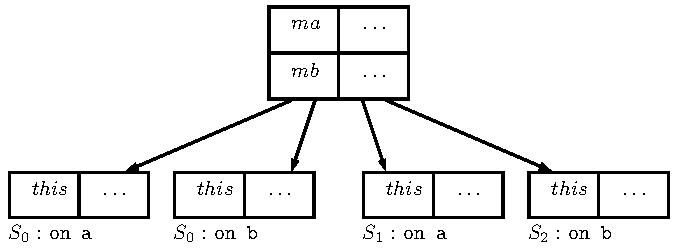
\includegraphics{figs/chapter_02_symtab_chain.pdf}
  \caption{Scoping structure of a synchroniser program using the zip2 synchroniser as an example}
  \label{fig:symtab_chain}
  \end{figure}

The symbol table implementation supports three operations: create a new symbol table, put a new entry in the table and get an entry for an identifier by searching the chain of tables starting with the table for the current transition. Later we refer to these operations as \emph{NewSymtab}(symtab), symtab.\emph{put}(\emph{ID, value}) and symtab.\emph{get}(\emph{ID}). The pseudo-code implementations of symtab.\emph{get} and symtab.\emph{put} are given in Fig. \ref{symtab_get} and Fig. \ref{symtab_put} respectively.

\begin{figure}[h!]
\noindent\fbox{%
\begin{minipage}{\dimexpr\linewidth-2\fboxsep-2\fboxrule\relax}
\begin{algorithmic}[1]
\Function{get}{$symtab, id$}
  \While{$symtab \; is \; not \; nil$}
    \State $tmp\gets get(symtab, id)$
    \If{$tmp$}
      \State \textbf{return} \emph{tmp}
    \Else
      \State $symtab\gets previous(symtab)$\Comment{\emph{previous(symtab)} returns a symbol table of the most-closely outer scope}
    \EndIf
  \EndWhile
  \State \textbf{return} \emph{not\_found}
\EndFunction
\end{algorithmic}
\end{minipage}%
}
\caption{Getting an entry for an identifier from the chained symbol table\label{symtab_get}}
\end{figure}

The synchroniser language restricts the reserved words to be identifiers (Appendix \ref{sync_kw}). An identifier is checked whether it is reserved when putting the entry in the symbol table.

\begin{figure}[h!]
\noindent\fbox{%
\begin{minipage}{\dimexpr\linewidth-2\fboxsep-2\fboxrule\relax}
\begin{algorithmic}[1]
\Function{put}{$symtab$, $id$, $value$}
  \If{\emph{id is reserved}}
    \State \emph{error}
  \EndIf
  \State $tmp\gets get(symtab, id)$
  \If{$not \; tmp$}
    \State $symtab\gets (id, value)$
  \Else
    \State \emph{error}
  \EndIf
\EndFunction
\end{algorithmic}
\end{minipage}%
}
\caption{Putting a new entry in the symbol table\label{symtab_put}}
\end{figure}



%Chaining of symbol tables results in a tree structure (probably we can simplity it somehow, because we do not really need a tree of scopes).

%The symbol table contains types and (possibly) locations. Builing of a symbol table Dragon book p.90.


\subsection{Semantic Analysis}
In addition to creating an intermediate representation, a compiler front end checks that the source program follows the syntactic and semantic rules of the source language. This checking is called static checking. It assures that certain kinds of programming errors, including type mismatched, are detected and reported during compilation.

Static checking includes:
\begin{itemize}
\item Syntactic checking. Constraints such as an identifier is declared at most once in a scope
\item Type checking. The type rules of a language assure that an operator or function is applied to the right number and type of operands.
\end{itemize}

  \subsubsection{Syntactic Checking}
In this section we describe the syntactic checks that are not enforced by the grammar.

The synchroniser language requires identifiers except for state expression aliases to be declared before they are used. Moreover, an identifier must be declared at most once in a scope. The channels, on which the transitions in the synchroniser are made, must be declared in the channel signature as well as the channels where messages are sent. In order to check it, we maintain three symbol tables for identifiers, input channels and output channels. The scheme given in Fig. \ref{synt_scheme} shows how the symbol tables are managed and used during the syntax analysis. The symbol tables are initialised before the syntax analyser runs, as shown in Fig. \ref{symtab_init}.

The attribute \emph{type} is added to each entry in the symbol table. State variables are assigned type \emph{integer}. Non-integer variables, whose structure is not known, are assigned a special type \emph{void}, which stands for a variable CAL term. A detailed information about the synchroniser language type system is provided in section \ref{type_check}.


\begin{figure}[h!]
\noindent\fbox{%
\begin{minipage}{\dimexpr\linewidth-2\fboxsep-2\fboxrule\relax}
\begin{algorithmic}
\Function{init}{}
    \State $InChantab\gets NewSymtab(nil)$
    \State $OutChantab\gets NewSymtab(nil)$
    \State $RootSymtab\gets NewSymtab(nil)$
\EndFunction
\end{algorithmic}
\end{minipage}%
}
\caption{Initialisation of symbol tables\label{symtab_init}}
\end{figure}



%\begin{figure}[h!]
\begin{sidewaystable}
\def\arraystretch{2} 
\begin{tabular*}{1\textwidth}{p{0.5\textwidth}|p{0.5\textwidth}}
\hline
Production & Semantic Action\\

\hline

\parbox{0.5\textwidth}{
\iangled{synch} ::= \tangled{synch} \iangled{ID} \tangled{(} \iangled{input} [\tangled{,} \iangled{input}]*

~~\tangled{|} \iangled{output} [\tangled{,} \iangled{output}]* \tangled{)} \tangled{\{} \iangled{decl}* \iangled{state}$^+$ \tangled{\}}
} & \parbox{0.5\textwidth}{
/* \emph{synch} holds the abstract syntax tree of the processed source code.  */
}\\

\hline

\parbox{0.5\textwidth}{
\iangled{input} ::= \iangled{chan} [\tangled{:} (\iangled{ID} $\mid$ \iangled{NUMBER})]

\iangled{chan} ::= \iangled{ID}
} & \parbox{0.5\textwidth}{
\emph{foreach} \iangled{chan}

~~InChantab.\emph{put}(\iangled{chan}, \emph{type=void})
}\\

\hline

\parbox{0.5\textwidth}{
\iangled{output} ::= \iangled{chan} [\tangled{:} \iangled{depth\_exp}]

\iangled{chan} ::= \iangled{ID}
} & \parbox{0.5\textwidth}{
\emph{foreach} \iangled{chan}

~~OutChantab.\emph{put}(\iangled{chan}, \emph{type=void})
}\\

\hline

\parbox{0.5\textwidth}{
\iangled{decl} ::= \tangled{store} \iangled{store\_id\_list} \tangled{;}

~~$\mid$ \tangled{state} \iangled{type} \iangled{state\_id\_list} \tangled{;}

\iangled{store\_id\_list} ::= \iangled{id\_list}

\iangled{state\_id\_list} ::= \iangled{id\_list}
} & \parbox{0.5\textwidth}{
\emph{foreach} \texttt{id} \emph{in} \iangled{store\_id\_list}

~~Symtab.\emph{put}(\texttt{id}, \emph{type=void})

\emph{foreach} \texttt{id} \emph{in} \iangled{state\_id\_list}

~~Symtab.\emph{put}(\texttt{id}, \emph{type=int})
}\\

\hline

\parbox{0.5\textwidth}{
\iangled{trans\_stmt} ::=

~~\iangled{trans\_name} [\tangled{.} \iangled{condition}] [\tangled{\&} \iangled{int\_exp} ] \iangled{actions}
} &\\

\hline

\parbox{0.5\textwidth}{
\iangled{trans\_name} ::= \iangled{ID}
} & \parbox{0.5\textwidth}{
\emph{if not} InChantab.\emph{get}(\iangled{ID})

~~\emph{error}

Symtab = NewSymtab(\emph{RootSymtab})

Symtab.\emph{put}(\tangled{this}, \emph{type=void})
}\\

\hline

\parbox{0.5\textwidth}{
\iangled{condition} ::= \tangled{@} \iangled{segmark}

~~$\mid$ \tangled{?} \iangled{ID}

~~$\mid$ \tangled{else}

\iangled{segmark} ::= \iangled{ID}
} & \parbox{0.5\textwidth}{
\emph{if not} Symtab.\emph{get}(\iangled{segmark})

~~\emph{error}
}\\

\hline

\parbox{0.6\textwidth}{
\iangled{condition} ::= [\tangled{?} \iangled{ID}] \tangled{(} \iangled{id\_list} [\tangled{||} \iangled{tail} ]\tangled{)}
} & \parbox{0.4\textwidth}{
\emph{foreach} \texttt{id} \emph{in} \iangled{id\_list} $\cap$ \iangled{tail}

~~Symtab.\emph{put}(\texttt{id}, \emph{type=void})

tmp = Symtab.\emph{get}(\tangled{this})

tmp.\emph{type} = \texttt{\{ \tangled{$p_1$}:\emph{void}, \dots \tangled{$p_n$}:\emph{void} \}}, where \emph{$p_1$, \dots $p_n$} are elements of \iangled{id\_list}

\emph{if} \iangled{tail}

~~tmp.\emph{type} = tmp.\emph{type} $\mid$ \iangled{tail}
}\\

\hline

\parbox{0.5\textwidth}{
\iangled{send\_stmt} ::= \tangled{send} \iangled{dispatch} [\tangled{,} \iangled{dispatch}* \tangled{;}

\iangled{dispatch} ::= \iangled{msg\_exp} \tangled{=>} \iangled{ID}
} & \parbox{0.5\textwidth}{
tmp = OutChantab.\emph{get}(\iangled{ID})

\emph{if not} tmp

~~\emph{error}
}\\

\hline
% goto is a state list, not a chan list
%\parbox{0.5\textwidth}{
%\iangled{goto\_stmt} ::= \tangled{goto} \iangled{id\_list} \tangled{;}
%} & \parbox{0.5\textwidth}{
%\emph{foreach} \texttt{id} \emph{in} \iangled{id\_list}
%
%~~\emph{if not} InChantab.\emph{get}.(\texttt{id})
%
%~~~~\emph{error}
%}\\
%
%\hline

\end{tabular*}
\caption{Symbol tables management and duplicate declaration checking scheme\label{synt_scheme}}
\end{sidewaystable}
%\end{figure}

%Check if all gotos point to existing states
The synchroniser compiler checks if the transition diagram of a synchroniser is closed. The algorithm given in Fig. \ref{goto_check} walks the abstract syntax tree \emph{synch} and constructs two sets: the set of the synchroniser state labels \emph{StateSet} and the set of the goto labels \emph{GotoSet}. The set $GotoSet \setminus StateSet$ contains goto labels that point to non-existent states. If this set is not empty the compilation fails with an error. The set $StateSet \setminus (GotoSet \cup \tangled{start})$ contains unreachable states that are eliminated. The algorithm also checks if the labels of the synchroniser states are unique.

A synchroniser program must have the state labeled \tangled{start}. The existence of this state is checked once the $StateSet$ is constructed.

\begin{figure}[h!]
\noindent\fbox{%
\begin{minipage}{\dimexpr\linewidth-2\fboxsep-2\fboxrule\relax}
\begin{algorithmic}[1]
\Function{get\_states}{$synch$}
  \State $StateSet\gets []$
  \State $GotoSet\gets []$
  \For{\textbf{each} \emph{state in state\_list(sync)}}
    \If{$label(state) \in StateSet$}
      \State \emph{error}\Comment{The state label is not unique}
    \Else
      \State $s\gets s$ \textbf{..} $label(state)$
    \EndIf

    \For{\textbf{each} \emph{trans in trans\_list(state)}}
      \For{\textbf{each} \emph{gotostate in goto\_list(trans)}}
        \If{$gotostate \notin GotoSet$}
          \State $GotoSet\gets GotoSet$ \textbf{..} $gotostate$
        \EndIf
      \EndFor
    \EndFor
  \EndFor
  \State \textbf{return} \emph{(StateSet, GotoSet)}
\EndFunction
\end{algorithmic}
\end{minipage}%
}
\caption{Construction of \emph{StateSet} and \emph{GotoSet}\label{goto_check}}
\end{figure}


%The synchroniser language supports configurable channel depth for input and output channels. If an input channel has the configurable depth, the depth of an output channel may be specified as an integer shift to the input channel depth. In other cases the shift is not needed.

%Channel signature. If the output channel depth is in the form of depth expression $p+integer$, then $p$ should be the depth of one of the input channels. $p$ is not allowed anywhere in state expressions.
%  \begin{itemize}
%  \item (a:p | b:p+1) - allowed
%  \item (a:p | b:0) - allowed
%  \item (a:p | b:r) - allowed
%  \item (a:p | b:r+1) - NOT allowed
%  \end{itemize}
%The special depth $-1$ indicated that the channel is not used. Therefore, if it is an input channel, all the transitions reading from it can be removed. If it is an output channel, and the transition that sends to this channel is valid, then an error must occur.


The synchroniser language provides two types of state variables: an integer of the specified width and a enumeration. The width defines the value range of an integer. The value range of a enumeration is specified in the variable declaration. Fig. \ref{int_range} gives the formulae for the value range computation.

%The width  decreases the number of possible states of a synchroniser. At low level state variables are machine- and target language- depedent integers.

\begin{figure}[h!]
\centering
\begin{tabular}{|c|c|}
\hline
Type & Values\\
\hline
$int(n)$ & $[0; 2^{n}-1] \cap \mathbb{Z}$\\
\hline
$enum(a_1$, $a_2$, $\dots$ $a_n)$ & $[0; n-1] \cap \mathbb{Z}$\\
\hline
$enum(a_1=N_1$, $a_2=N_2$, $\dots$ $a_n=N_n)$ & $N_1$, $N_2$, $\dots$ $N_n$\\
\hline
\end{tabular}
\caption{Computing the value range of an integer variable\label{int_range}}
\end{figure}

For state expressions that evaluate to integer values we can check if the computed value fits in the assignment destination value range. The symbol table stores the value range information for integer entries and provides the interface to access it in a form of boolean function \texttt{check\_range}(\emph{id}, \emph{value}). The function returns \emph{true} if \emph{value} fits in the \emph{id} value range and \emph{false} otherwise. Fig. \ref{ts_stmt} shows how the check is integrated into the syntax analyser.

%Check if the range condition is valid at least for assignments (int(1) x = 10 is not good, should issue a warning, check what would be assigned to x in C). For the state expressions that evaluate during the execution of the synchroniser it's probably ok to delegate the overflow checks to the C compiler.

%The grammar for integer expression used in our implementation of a synchroniser compiler (Appendix \ref{int_exp_gr}) is a simplified version of the C grammar for arithmetic expression.

%TODO fix!
    \paragraph{Tests}
We have developed the testing package for the semantic analyser. It uses standard python unittest module. The testing is based on expanding the abstract syntax tree into a nested list.


  \subsubsection{Type Checking\label{type_check}}
Static type checking is the process of verifying the type safety of a program based on analysis of the program's source code. If a program passes a static type checker, then the program is guaranteed to satisfy some set of type safety properties for all possible inputs.

The design of a type checker is based on information about the syntactic constructs in the language, the notion of types and the rules for assigning types to language constucts. The type of a language construct is denoted by a type expression. Informally, a type expression is either a basic type or is formed by applying an operator called a type constructor to other type expressions. A collection of rules for assigning type expressions to language constructs is called a type system.

%A language is strongly typed if a compiler can garantee that the programs it accepts will execute without type errors.
%The language in which identifiers must be declared before they are used.
The communication protocol of the \ak\ runtime system prototype supports only records. We implement the type system of the synchroniser language taking this fact into account. The basic types in the synchroniser language are integers and CAL variable terms. Integer is the type of state variables. Variable terms are building blocks for the only constructed type in the synchroniser language -- a record. A record is constructed by the catenation of two records. The pseudo-code of the record constructor $||$ is given in Fig. \ref{rec_construc}. The record constructor is obviously commutative and associative.

\begin{figure}[h!]
\noindent\fbox{%
\begin{minipage}{\dimexpr\linewidth-2\fboxsep-2\fboxrule\relax}
\begin{algorithmic}[1]
\Function{$||$}{$r_1, \; r_2$}
  \If{$len(r_1)\le len(r_2)$}
    \State $r_{iter}\gets r_1$
    \State $r\gets r_2$
  \Else
    \State $r_{iter}\gets r_2$
    \State $r\gets r_1$
  \EndIf\Comment{\emph{$r$ is the record that contains fewer label-value pairs}}

  \For{\textbf{each} \emph{label-value pair (l,v) in} $r_{iter}$}
    \If{$r(l)$}\Comment{\emph{if label l exists in r}}
      \State $r(l)\gets union(r(l),v)$
    \Else
      \State $r(l)\gets v$
    \EndIf
  \EndFor
  \State \textbf{return r}
\EndFunction
\end{algorithmic}
\end{minipage}%
}
\caption{The record type constructor $||$\label{rec_construc}}
\end{figure}

The case when a label-value pair labeled $l$ exists in both operand records $r_1$ and $r_2$ is indicated with $union(r_1(l),r_2(l))$. The CAL solver resolves which option to take during the constraint aggregation pass in the \ak\ compiler.
%When labels intersect, it is the deal for CAL solver to resolve with option to take (it should consider flow inheritance).

We describe the type systems in terms of grammar productions and corresponding semantic actions. The type systems for state and store expressions is given in Fig. \ref{ts_int_exp} and Fig. \ref{ts_data_exp} respectively. The synthesized attribute \emph{type} for an expression \iangled{E} gives the type of the expression assigned by the type system for the expression generated by \iangled{E}. The type system for statements is given in Fig. \ref{ts_stmt}. It assures that the left hand side can be assigned to.


\begin{figure}[h!]
%\begin{sidewaystable}
\def\arraystretch{2} 
\begin{tabular*}{1\textwidth}{p{0.5\textwidth}|p{0.5\textwidth}}
\hline
Production & Semantic Action\\

\hline

\parbox{0.5\textwidth}{
\iangled{assign} ::= \iangled{dest} \tangled{=} \tangled{[} \iangled{int\_exp\_c} \tangled{]}

\iangled{dest} ::= \iangled{ID}
} & \parbox{0.5\textwidth}{
tmp = Symtab.\emph{get}(\iangled{dest})

\emph{if not} tmp

~~Symtab.\emph{put}(\iangled{dest}, \emph{type=int})

\emph{else}

~~\emph{if} tmp.\emph{type} != \emph{int}

~~~~\emph{error}

~~\emph{if} \iangled{int\_exp\_c} \emph{evaluates to int}

~~~~\emph{if not check\_range}(\iangled{dest}, \emph{eval}(\iangled{int\_exp\_c}))

~~~~~~\emph{error}
}\\

\hline

\parbox{0.5\textwidth}{
\iangled{assign} ::= \iangled{dest} \tangled{=} \iangled{data\_exp}

\iangled{data\_exp} ::=

~~(\iangled{data} $\mid$ \tangled{(} \iangled{data} \tangled{)})

} & \parbox{0.5\textwidth}{
tmp = Symtab.\emph{get}(\iangled{dest})

\emph{if not} tmp

~~\emph{error}

\emph{if} tmp.\emph{type == int}

~~\emph{error}

tmp.\emph{type} = \iangled{data\_exp}.\emph{type}
}\\

\hline

\end{tabular*}
\caption{Type system for statements\label{ts_stmt}}
%\end{sidewaystable}
\end{figure}



\begin{figure}[h!]
%\begin{sidewaystable}
\def\arraystretch{2} 
\begin{tabular*}{1\textwidth}{p{0.5\textwidth}|p{0.5\textwidth}}
\hline
Production & Semantic Action\\

\hline

\parbox{0.5\textwidth}{
\iangled{int\_exp\_c} ::= \iangled{NUMBER} $\mid$ \iangled{ID}
} & \parbox{0.5\textwidth}{
tmp = Symtab.\emph{get}(\iangled{ID})

\emph{if not} tmp

~~\emph{error}

\emph{if} tmp.\emph{type != int}

~~\emph{error}

\iangled{int\_exp\_c}.\emph{type} = \emph{int}
}\\

\hline

\parbox{0.5\textwidth}{
\iangled{int\_exp\_c} ::= \tangled{(} \iangled{$int\_exp\_c_{1}$} \tangled{)}

~~$\mid$ \tangled{-} \iangled{$int\_exp\_c_{1}$}

~~$\mid$ \tangled{!} \iangled{$int\_exp\_c_{1}$}
} & \parbox{0.5\textwidth}{
\iangled{int\_exp\_c}.\emph{type} = \iangled{$int\_exp\_c_{1}$}.\emph{type}
}\\

\hline

\parbox{0.5\textwidth}{
\iangled{int\_exp\_c} ::=

~~~~\iangled{$int\_exp\_c_{1}$} \iangled{op} \iangled{$int\_exp\_c_{2}$}

\iangled{op} ::= \tangled{+} $\mid$ \tangled{-} $\mid$ \tangled{*} $\mid$ \tangled{/} $\mid$ \tangled{\%}

~~$\mid$ \tangled{<<} $\mid$ \tangled{>>} $\mid$ \tangled{|} $\mid$ \tangled{\&} $\mid$ \tangled{\textasciicircum}

~~$\mid$ \tangled{<} $\mid$ \tangled{>} $\mid$ \tangled{==} $\mid$ \tangled{!=} $\mid$\tangled{<=}

~~$\mid$ \tangled{>=} $\mid$ \tangled{\&\&} $\mid$ \tangled{||}
} & \parbox{0.5\textwidth}{
\emph{if} \iangled{$int\_exp\_c_{1}$}.\emph{type} == \emph{int}

~~\emph{and} \iangled{$int\_exp\_c_{2}$}.\emph{type} == \emph{int}

~~\iangled{int\_exp\_c}.\emph{type} = \emph{int}

\emph{else}

~~\emph{error}
}\\

\hline

\end{tabular*}
\caption{Type system for state expressions\label{ts_int_exp}}
%\end{sidewaystable}
\end{figure}


\begin{figure}[h!]
%\begin{sidewaystable}
\def\arraystretch{2} 
\begin{tabular*}{1\textwidth}{p{0.5\textwidth}|p{0.5\textwidth}}
\hline
Production & Semantic Action\\

\hline

\parbox{0.5\textwidth}{
\iangled{data} ::= \iangled{item\_list}

\iangled{item\_list} ::= \iangled{item} [\tangled{||} \iangled{item}]*
} & \parbox{0.5\textwidth}{
\emph{foreach} \texttt{item} \emph{in} \iangled{item\_list}

~~\iangled{data}.\emph{type} = \iangled{data}.\emph{type} $||$ \texttt{item}.\emph{type}
}\\

\hline

\parbox{0.5\textwidth}{
\iangled{item} ::= \tangled{this}
} & \parbox{0.5\textwidth}{
tmp = Symtab.\emph{get}(\tangled{this})

\iangled{item}.\emph{type} = tmp.\emph{type}
}\\

\hline

\parbox{0.5\textwidth}{
\iangled{item} ::= \iangled{ID}
} & \parbox{0.5\textwidth}{
tmp = Symtab.\emph{get}(\iangled{ID})

\emph{if not} tmp

~~\emph{error}

\emph{if} tmp.\emph{type == int}

~~\emph{error}

\iangled{item}.\emph{type} = tmp.\emph{type}
}\\

\hline

\parbox{0.5\textwidth}{
\iangled{item} ::= \tangled{'} \iangled{ID}
} & \parbox{0.5\textwidth}{
tmp = Symtab.\emph{get}(\iangled{ID})

\emph{if not} tmp

~~\emph{error}

\iangled{item}.\emph{type} = \{ \tangled{ID}:tmp.\emph{type} \}
}\\

\hline

\parbox{0.5\textwidth}{
\iangled{item} ::= \iangled{ID} \tangled{:} \iangled{rhs}

\iangled{rhs} ::= \iangled{int\_exp} $\mid$ \iangled{rhs\_ID}

\iangled{rhs\_ID} ::= \iangled{ID}
} & \parbox{0.5\textwidth}{
\emph{if} \iangled{rhs\_ID}

~~tmp = Symtab.\emph{get}(\iangled{rhs\_ID})

~~\emph{if not} tmp

~~~~\emph{error}

tmp = Symtab.\emph{get}(\iangled{ID})

\iangled{item}.\emph{type} = \{ \tangled{ID}:\iangled{rhs}.\emph{type} \}
}\\

\hline

\end{tabular*}
\caption{Type system for store expressions\label{ts_data_exp}}
%\end{sidewaystable}
\end{figure}

%If an identifier was met and it is already in the current scope of symbol table, it must have the same type (int or data) as before.


%\subsection{Code optimisation}
%Code optimiser is a framework for writing optimisation passes, which currently has only dead code elimination. 
%
%  \paragraph{Dead code elimination}
%\begin{itemize}
%\item Remove unreachable states of an automaton (when there's no state variables involved).
%
%\item Remove unreachable transitions based on Section Execution order.
%
%\item Remove unused state, store variables and assignments (this may require some simple def-use analysis, probably can put it into symbol tables).
%\end{itemize}


\subsection{Code generation}
  \paragraph{Synchroniser runtime code}
%Give a class diagram?
%Generator architecture - node visitor

  \paragraph{Synchroniser passport}
A synchroniser can impose some restriction on the type of messages it accepts.
In the implementation we consider that only choices travel between channels (it is unclear what is a unification of lists, how to order the elements in the resulting list).

In the implementation we restrict to choices and records.

None indicates that it is a term variable.


Input channels: Fig. \ref{a}.
We have types of 'this' for each output channel.
Need to walk the transitions to find all 'this' types that belong to the same channel and then unify them.
\begin{figure}[h!]
\begin{lstlisting}
//term: None (term variable), Int, Record, Choice
a.(x,y||t) {
  //x - is a value not a pair. In a store expression of in a send it must be 'x
  //term(x) = None
  //term(y) = None
  //term(this) = { x:term(x), y:term(y) | $t }
  //term(a) = (: uniq:term(this) :)

  set n = [x];
  //term(x) = Int
  //term(this) = { x:term(x), y:term(y) | $t }
}

a.?v(x,y||t) {
  //term(x) = None
  //term(y) = None
  //term(this) = { x:term(x), y:term(y) | $t }    //why not a list/tuple/choice as well?
  //term(a) = (: v:term(this) | $a_t :)           //because it's unclear how to unify ordered structures?

  set n = [x];
  //term(x) = Int
  //term(a) = (: v:{ x:term(x), y:term(y) | $t } | $a_t :)
}
\end{lstlisting}
\label{a}
\end{figure}

Output channels: Fig. \ref{b}.
How is the type of the output channel computed? Give algorithm for 'send' clause.
Find all sends to the particular channel.
Walk the variables in every 'send' clause (their types are know) and unify them.
\begin{figure}[h!]
\begin{lstlisting}[frame=single]
//record union with label 'x' collision: {x:type_1, y:...} + {x:type_2, z:...} = {x:union(type_1,type_2), y:..., z:...}
//python's dict.update(...)
a.(x,y||t) {
  //term(x) = None
  //term(y) = None
  //term(this) = { x:term(x), y:term(y) | $t }
  //term(a) = (: uniq:term(this) :)

  set ma = (this || id:y);
  //term(ma) = term(this) || id:term(y) =
             = { x:term(x), y:term(y), id:term(y) | $t }

  send ?v(ma || n:x) => c, send this => d;
  //term(c) = (: v:(term(ma) || n:x) | $c_t :) =
            = (: v:{ x:term(x), y:term(y), id:{ y:term(x) }, n:term(x) | $t } | $c_t :)

  //term(d) = (: uniq:term(this) :)
}
\end{lstlisting}
\label{b}
\end{figure}


\section{Discussion}
Optimisations based on execution order: remove unreachable transitions.

MDL is wider than what the presented synchroniser can synchronise. TODO: give examples. However, it need to be elaborated with the real world applications of \ak\ whether it is useful to implement it in synchronisers.

Decide how to do flow inheritance in synchronisers. This will be done outside of synchronisers. Need to somehow specify which fields are inherited and which are not. In synchroniser transitions we can pick fields of an accepted message, with ehich we want to do something in synchroniser. However, there may be many fields in the message and some of them do not need to be inherited. In theory we could pick all the fields that we want to inherit along with the fields we want to work with, and them concat them and send them to then output channel. But there may be too many to specify manually for eack transition in the synchroniser caused by the channel.
